\section{Results}
\label{sec:results}

This section presents the validation of the joint friction torque estimation using the PINN and compares it with the CV and SCV models discussed in Section~\ref{sec:cv_scv}. We evaluate the performance of these models on the left ankle roll and left knee joints of the ergoCub humanoid robot (Fig. \ref{fig:ergocub} and ~\ref{fig:ankleext}). These joints are selected due to their distinct characteristics: the ankle roll joint has minimal load and is predominantly influenced by frictional forces, making friction compensation critical for precise control, while the knee joint experiences varying load conditions that affect friction differently depending on the leg configuration. We employ the high-level controller outlined in Section~\ref{sec:HLC} to track desired joint position trajectories. This controller generates the desired torque commands, which are then sent to the low-level joint torque controller. The low-level controller uses friction torque estimates from the friction models to provide compensation. The friction torque estimator is seamlessly integrated within the robot computer, operating automatically at a frequency of $1000$ Hz upon startup. Two distinct experiments are conducted to assess the effectiveness of the friction models, and the results are also showcased in the supplementary video. The code is available online~\cite{code}.
\looseness=-1

\begin{figure}[t]
\centering
\begin{subfigure}{.98\columnwidth}
  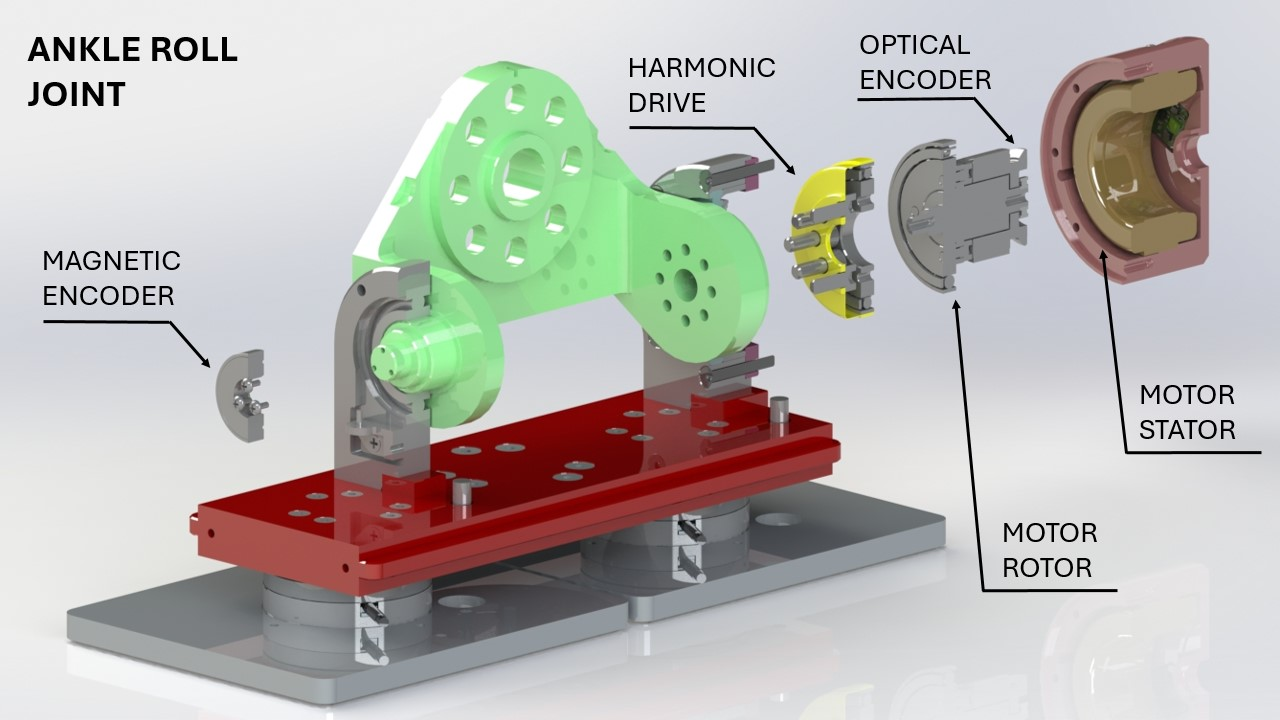
\includegraphics[width=\textwidth]{figures/ankleroll.jpg}
\end{subfigure}%
\vspace{5pt} % Add horizontal space between subfigures
\begin{subfigure}{.98\columnwidth}
  \includegraphics[width=\textwidth]{figures/ankle_ergocub_extcontact.png}
\end{subfigure}
\caption{Exploded view of the ankle roll joint and left ankle roll while applying external disturbances.}
\label{fig:ankleext}
\vspace{-15pt}
\end{figure}

\subsection{CV and SCV models identification}
\label{sec:whitebox}

We utilized a data-driven approach to identify the parameters of the CV and SCV models using experimental data. The optimization process aims to minimize the mean squared error (MSE) between the predicted and measured friction torques,
\mbox{$\text{MSE} = \frac{1}{N} \sum_{i=1}^{N} ({\tau_{F, \text{pred}_i}} - {\tau_{F, \text{true}_i}})^2$}.
 The Adam optimizer, applied over $10000$ epochs, adjusts the model parameters such as $k_a$, $k_c$ and $k_v$ for the CV model~\eqref{eq:cv}, and $v_s$, $k_a$, $k_c$, $k_v$ and $\alpha$ for the SCV model~\eqref{eq:scv}. Both models used joint velocity data $\dot{s}$ as input and friction torque $\tau_F$ as the target output. Once trained, these parameters are employed for friction compensation in the low-level controller. The resulting parameters are listed in~\ref{table:cvscv}.
\looseness=-1

\subsection{PINN hyperparameter identification}

\begin{table}[t]
\centering
\caption{Identified parameters for the Coulomb-viscous (CV) and Stribeck-Coulomb-viscous (SCV) friction models.}
\setlength{\tabcolsep}{4pt}
\begin{tabular}{lcccc}
\hline
\textbf{Parameters} & $\text{CV}_{\text{ankle\_roll}}$ & $\text{SCV}_{\text{ankle\_roll}}$ & $\text{CV}_{\text{knee}}$ & $\text{SCV}_{\text{knee}}$ \\ 
\hline
$k_a$ [\SI{}{s\per rad}] & 10.53 & 2.78 & 50.8400 & 16.95 \\ 
$k_c$ [\SI{}{Nm}] & 1.2 & 1.0005 & 8.1 & 5.0 \\ 
$k_v$ [\SI{}{Nm.rad\per\second}] & 0.24 & 0.29 & 5.55 & 5.34 \\ 
$k_s$ [\SI{}{Nm}] & - & 6.0 & - & 9.7 \\ 
$v_s$ [\SI{}{rad\per\second}] & - & 0.13 &  -  & 5.4 \\ 
$\alpha$ & - & 0.6 & - & 0.5 \\
\hline
\label{table:cvscv}
\vspace{-15pt}
\end{tabular}
\end{table}
\looseness=-1

The hyperparameters of the PINN model are identified using the Weight and Biases tool~\cite{wandb}. Table~\ref{table:hyper} presents the optimal hyperparameters identified, with training taking approximately one hour and a half per run. The training loss for the ankle roll joint is $0.0044$, with a validation loss of $0.000878$, whereas for the knee joint, the training and validation losses are $0.323$ and $0.0787$, respectively.
\looseness=-1

\begin{figure*}[t]
\centering
\begin{subfigure}{.49\textwidth}
  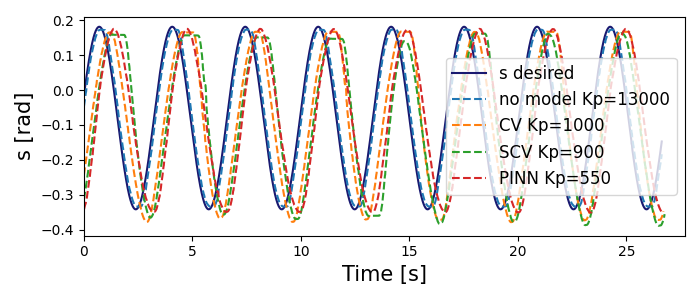
\includegraphics[width=0.98\linewidth,center]{figures/sinusoid_tracking_high_kp.png}
  \vspace{-20pt}
  \caption{Joint position tracking.}
  \label{fig:kptrackingankle}
\end{subfigure}%
\hspace{\fill} % Add horizontal space between subfigures
\begin{subfigure}{.49\textwidth}
  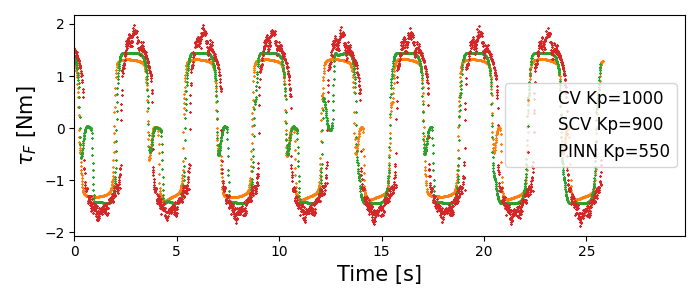
\includegraphics[width=0.98\linewidth,center]{figures/friction_high_kp.png}
  \vspace{-20pt}
  \caption{Estimated friction torques.}
  \label{fig:kpfrictionankle}
\end{subfigure}
\begin{subfigure}{.98\textwidth}
  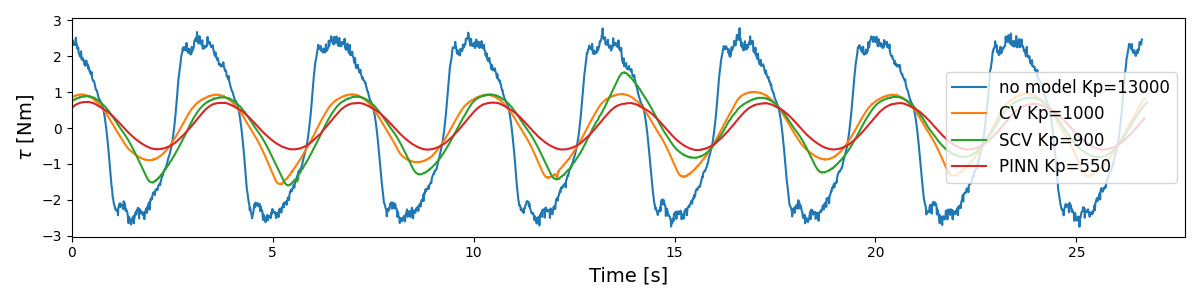
\includegraphics[width=0.9\linewidth,center]{figures/torque_sinusoid_tracking_high_kp_2.png}
  \vspace{-20pt}
  \caption{Desired joint torques.}
  \label{fig:kptorqueankle}
\end{subfigure}
\vspace{-5pt}
\caption{Left ankle roll results. Comparison of joint position tracking, friction estimation, and desired joint torques with different high-level control gains tuned on each specific friction model.}
\vspace{-10pt}
\end{figure*}
\begin{figure*}[t]
\centering
\begin{subfigure}{.48\textwidth}
  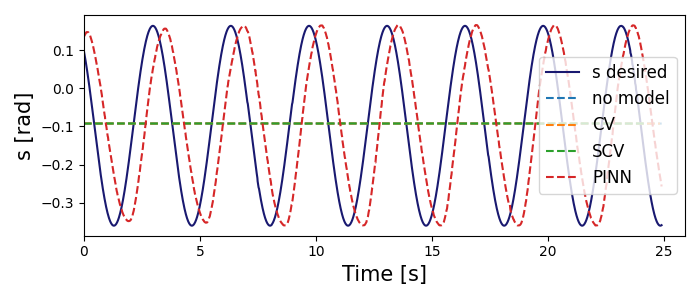
\includegraphics[width=0.98\linewidth,center]{figures/sinusoid_tracking.png}
  \vspace{-20pt}
  \caption{Joint position tracking.}
  \label{fig:kp550trackingankle}
\end{subfigure}%
\hspace{\fill} % Add horizontal space between subfigures
\begin{subfigure}{.48\textwidth}
  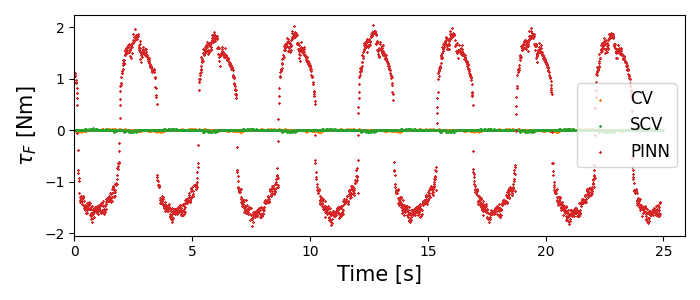
\includegraphics[width=0.98\linewidth,center]{figures/friction_kp_550.png}
  \vspace{-20pt}
  \caption{Estimated friction torques.}
  \label{fig:kp550frictionankle}
\end{subfigure}
\vspace{-5pt}
\caption{Left ankle roll results. (a)-(b) Comparison of the joint position tracking and estimated friction $K_p=550$ and $K_d=4$.}
\vspace{-15pt}
\end{figure*}

\begin{table}[t]
\centering
\caption{Physics Informed Neural Network hyperparameters identified using the Weight and Biase tool.}
\begin{tabular}{p{0.5\linewidth}cc}
\hline
\textbf{Hyperparameter} & \textbf{ankle\_roll} & \textbf{knee} \\
\hline
Epochs                  & 350  &  350    \\
Batch size              & 4316  &  4914   \\
Dropout rate            & 0.07  &  0.01176  \\
Hidden neurons layer 1     & 268  & 194  \\
Hidden neurons layer 2     & 215  & 247  \\
History length          & 20    &  22  \\
Learning rate           & 0.00076  & 0.00076 \\
$\lambda$               & 0.164  &  0.484 \\
Weight and biases initialization   & Random & Random \\
Optimizer & ADAM & ADAM \\
\hline
\label{table:hyper}
\end{tabular}
\vspace{-25pt}
\end{table}
\looseness=-1

\subsection{System performance with different friction models}
We evaluate the tracking performance of the friction models by having the left ankle roll and left knee joints follow a sinusoidal trajectory. The ergoCub's root link is fixed, allowing free motion of the legs. The high-level controller generates desired torque commands, which are transmitted to the feedforward low-level torque controller that integrates friction compensation from the respective models.

We conduct repeated experiments using various friction models, including a case without friction compensation. To assess the impact of each friction model, we identified the minimum proportional gain $K_p$ required to track the desired trajectory accurately. The $K_d$ gain is set to $4$ and is never changed.  A lower $K_p$ indicates more effective friction compensation, allowing for precise tracking with minimal control effort. Fig.~\ref{fig:kptrackingankle} compares the performance of the high-level controller adopting the three different friction models on the ankle roll joint. The PINN model achieves the lowest $K_p$, followed by the SCV and CV models. Similar trends are observed for the knee joint, as depicted in Fig.~\ref{fig:trackingknee}. The superior performance of the PINN model in requiring the lowest $K_p$ underscores its effectiveness in accurately estimating and compensating for friction. Fig.~\ref{fig:kpfrictionankle} and \ref{fig:frictionknee} present the friction estimated during the experiments described above, while Fig.~\ref{fig:kptorqueankle} depicts the relationship between $K_p$ values and the corresponding desired torques. In Figure \ref{fig:kptorqueankle} we observe that higher $K_p$ values correspond to higher desired torques, reflecting increased control effort needed for precise joint movement. This highlights the PINN model's efficiency in minimizing control effort by accurate friction compensation. Conversely, the knee joint dynamics are primarily influenced by varying load rather than friction, making it less sensitive to $K_p$ adjustments (see Figure \ref{fig:torqueknee}). Overall, the significant disparity in desired torque values between no-compensation and friction-compensation cases is evident for both ankle roll and knee joints.
\looseness=-1

\begin{figure*}[t]
\centering
\begin{subfigure}{.49\textwidth}
  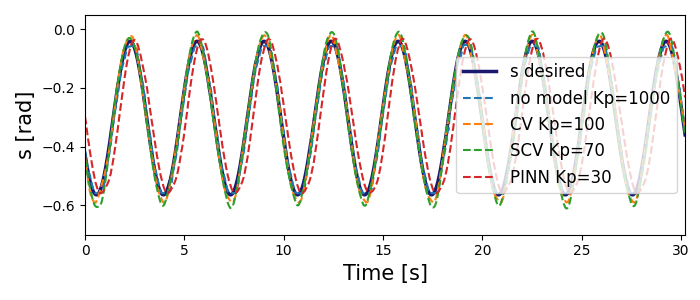
\includegraphics[width=0.98\linewidth,center]{figures/knee_sinusoid_tracking_highkp.png}
  \vspace{-20pt}
  \caption{Joint position tracking.}
  \label{fig:trackingknee}
\end{subfigure}%
\hspace{\fill} % Add horizontal space between subfigures
\begin{subfigure}{.49\textwidth}
  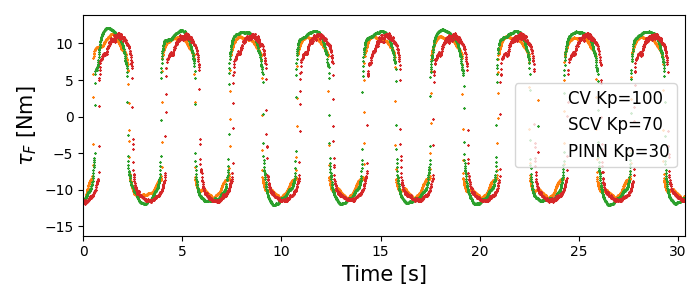
\includegraphics[width=0.98\linewidth,center]{figures/knee_friction_highkp.png}
  \vspace{-20pt}
  \caption{Estimated friction torques.}
  \label{fig:frictionknee}
\end{subfigure}
\begin{subfigure}{.98\textwidth}
  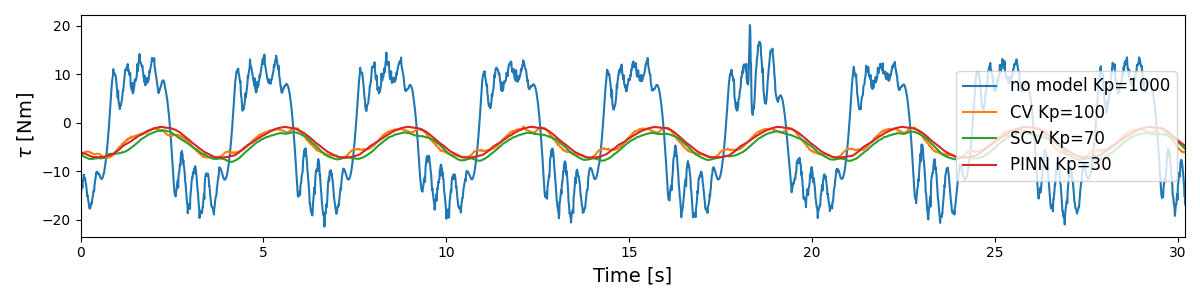
\includegraphics[width=0.9\linewidth,center]{figures/knee_torque_sinusoid_tracking_highkp.png}
  \vspace{-20pt}
  \caption{Desired joint torques.}
  \label{fig:torqueknee}
\end{subfigure}
\vspace{-5pt}
\caption{Left knee results. Comparison of joint position tracking, friction estimation, and desired joint torques with different high-level control gains tuned on each specific friction model.}
\vspace{-10pt}
\end{figure*}
\begin{figure*}[t]
\centering
\begin{subfigure}{.48\textwidth}
  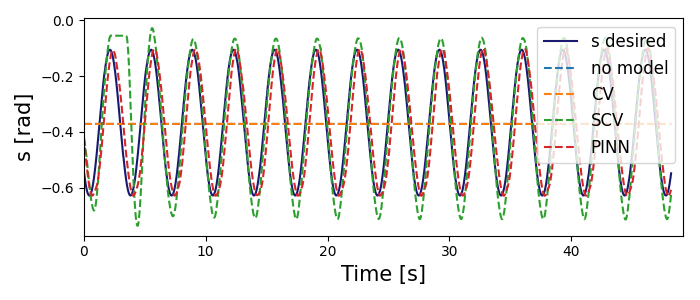
\includegraphics[width=0.98\linewidth,center]{figures/knee_sinusoid_tracking_kp30.png}
  \vspace{-20pt}
  \caption{Joint position tracking.}
  \label{fig:kp30trackingknee}
\end{subfigure}%
\hspace{\fill} % Add horizontal space between subfigures
\begin{subfigure}{.48\textwidth}
  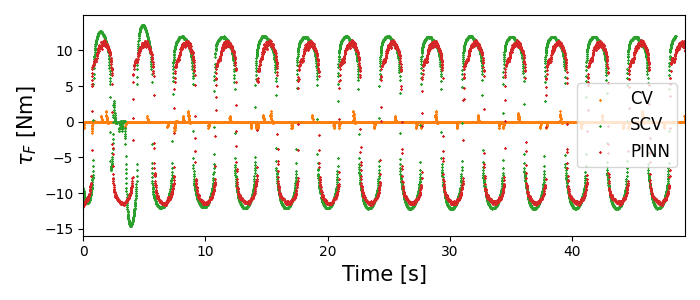
\includegraphics[width=0.98\linewidth,center]{figures/knee_friction_kp30.png}
  \vspace{-20pt}
  \caption{Estimated friction torques.}
  \label{fig:kp30frictionknee}
\end{subfigure}
\vspace{-5pt}
\caption{Left knee results. (a)-(b) Comparison of the joint position tracking and estimated friction with $K_p=30$ and $K_d=4$.}
\vspace{-15pt}
\end{figure*}

Fig.~\ref{fig:kptrackingankle} and Fig.~\ref{fig:trackingknee} show that systems with lower $K_p$, particularly those utilizing the PINN model, exhibit slight delays in joint position tracking, likely due to the less aggressive control action. In contrast, systems with higher gains, which lack proper friction compensation, generate higher desired torques and reduced tracking delays. Indeed, higher gains yield more aggressive responses, reducing the error between desired and actual joint positions. Introducing a feedback controller at the torque control level could combine the benefits of accurate friction compensation with improved tracking performance through feedback.
\looseness=-1

We also test the models using the lowest $K_p$ determined by the PINN-based friction estimation. The results show that the CV and SCV models are unable to generate sufficient torque to overcome static friction in the ankle roll joint, as shown in Fig.~\ref{fig:kp550trackingankle} and~\ref{fig:kp550frictionankle}. Conversely, for the knee joint, only the CV model fails to move the joint. However, the SCV model presents a higher tracking error for the sinusoidal trajectory compared to the PINN model, as evidenced in Fig.~\ref{fig:kp30trackingknee} and~\ref{fig:kp30frictionknee}, confirming the superior performance of the PINN model.
\looseness=-1

\subsection{Joint position stability and response to external wrenches}

\begin{table}[t]
\centering
\caption{Comparison of the results with different friction models for the left ankle roll joint.}
\setlength{\tabcolsep}{7pt}
\begin{tabular}{lcccc}
    \toprule
    Models    & RMSE [rad] & $\|\prescript{roll}{}{\mu_x}\|$ [Nm] & $K_p$ & $K_d$ \\
    \midrule
    No Model  & 0.009 & 21  & 13000 & 4 \\
    CV        & 0.05  & 4.7   & 1000 & 4 \\
    SCV       & 0.047 & 5.0   & 900 & 4  \\
    PINN      & 0.046 & 3.0   & 550 & 4  \\
    \bottomrule
\end{tabular}
\vspace{-12pt}
\label{tab:comparisonankle}
\end{table}
\begin{table}[t]
\centering
\caption{Comparison of the results with different friction models for the left knee joint.}
\setlength{\tabcolsep}{7pt}
\begin{tabular}{lcccc}
    \toprule
    Models    & RMSE [rad] & $\|\prescript{roll}{}{\mu_x}\|$ [Nm] & $K_p$ & $K_d$ \\
    \midrule
    No Model  & 0.0085 & 65.4  & 1000 & 4 \\
    CV        & 0.035  & 17.6   & 100 & 4 \\
    SCV       & 0.049 & 23.0   & 70 & 4  \\
    PINN      & 0.017 & 8.9   & 30 & 4  \\
    \bottomrule
\end{tabular}
\vspace{-20pt}
\label{tab:comparisonknee}
\end{table}
\looseness=-1
In our second experiment, we employ a high-level controller to maintain a fixed initial joint position under two distinct conditions: using the lowest $K_p$ values for all friction models and using $K_p$ values that demonstrated effective tracking in previous tests. This experiment aims to analyze the system response to an external disturbance and evaluate the efficacy of different friction models. As shown in Fig.~\ref{fig:ankleext}, the external disturbance is manually applied to attempt rotation of the joint about its rotation axis. This applied wrench is measured by two force/torque sensors positioned under the robot foot. The wrench is composed of three forces and three moments, but only one component directly influences the joint movement, while others are absorbed by the mechanical structure. To compute the disturbance wrench acting on the joint, we transform the measured wrench $\prescript{}{}{\mathrm{f}}_{measured}$ into a frame attached to the joint and whose \textit{x}-axis is aligned with the joint rotation axis, namely $f_{joint} = \prescript{joint}{}{X}_{measured} f_{measured}$. Finally, we extract from $f_{joint}$ only the moment about the \textit{x}-axis contributing to the joint rotation.
\looseness=-1

Using the $K_p$ values that provided good tracking in the previous tests, the results are summarized in Tables~\ref{tab:comparisonankle} and Table~\ref{tab:comparisonknee} for the two joints. The tables present the root mean square error (RMSE) of the joint position after the external disturbance ceased and the joint returned to the initial position. The tables also include the value of the external torque applied to the joint to move it from its initial position. 
\looseness=-1

When using the lowest $K_p=550$ for the ankle roll joint and $K_p=30$ for the knee joint, we observe that after the external disturbance is removed, the joint successfully returns to its starting position only when the PINN model is used as shown in Table~\ref{tab:comparisonlowkp}. For other friction models, the compensation is insufficient, and the desired torque generated by the controller is not enough to bring the joint back to its initial position. This indicates that the PINN model provides superior friction compensation, ensuring accurate joint position recovery even with a lower proportional gain.
\looseness=-1

\begin{table}[t]
\centering
\caption{Joint position tracking error after applying external disturbance while using different friction models and the same high-level controller gains.}
\setlength{\tabcolsep}{8pt}
\begin{tabular}{lcccc}
    \toprule
    & \textbf{No Model} & \textbf{CV} & \textbf{SCV} & \textbf{PINN} \\
    \midrule
    \textbf{Left Ankle Roll} & & & & \\
    RMSE [rad] & 0.19 & 0.2  & 0.21 & 0.046 \\
    $K_p=550$, $K_d=4$ & & & & \\
    \midrule
    \textbf{Left Knee} & & & & \\
    RMSE [rad] & 0.21  & 0.11   & 0.097 & 0.017 \\
    $K_p=30$, $K_d=4$ & & & & \\
    \bottomrule
\end{tabular}
\vspace{-15pt}
\label{tab:comparisonlowkp}
\end{table}

While a higher $K_p$ generally resulted in a lower RMSE, indicating better tracking accuracy, especially for the ankle roll joint, it also highlighted the drawbacks. Indeed, the lowest force is required with the lowest $K_p$. This observation underscores the benefits of accurate friction compensation. By accurately modeling and compensating for frictional forces, the joint requires less external torque to achieve desired movements. This not only enhances control precision but also minimizes mechanical stress and energy consumption, contributing to overall system efficiency and reliability.
\looseness=-1